\section*{Disk-unware (list) filesys has poor performance}
\begin{itemize}
\item Thompson wrote the 1st simple filesys for Unix: \textbf{S}uperblock with info about entire filesys and most disk space taken up by data blocks
\item support files and directory-based hierarchy, easy-to-use
\item terrible performance: 2\% of overall disk bandwidth; worse over time
\end{itemize}
\begin{minipage}{.5\linewidth}
  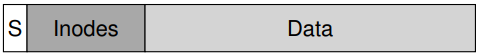
\includegraphics[width=\linewidth]{imgs/ffs_list1}
\end{minipage}
\begin{minipage}{.5\linewidth}
  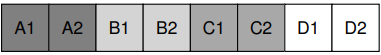
\includegraphics[width=\linewidth]{imgs/ffs_list2}
\end{minipage}
\begin{minipage}{.5\linewidth}
  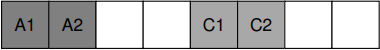
\includegraphics[width=\linewidth]{imgs/ffs_list3}
\end{minipage}
\begin{minipage}{.5\linewidth}
  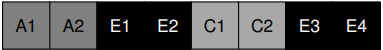
\includegraphics[width=\linewidth]{imgs/ffs_list4}
\end{minipage}
\begin{itemize}
\item main issue: treat disk like RAM; data spread all over the place; expensive positioning costs: data blks far away from its inode $\to T_{\text{seek}} \uparrow$
\item fragmentation: logically contiguous file accessed across the disk
\item defragmentation tools reorganize on-disk data to place files contiguously and make free space for $\geq 1$ contiguous regions
\item another issue: original block size too small (512 bytes) $\to$ transferring data from the disk was inherently inefficient: smaller blks minimizes internal fragement but bad for transfer $\because$ positioning overhead
\end{itemize}
\section*{FFS: Disk-Aware, Cylinder/Blk Groups (same API, diff. internal)}
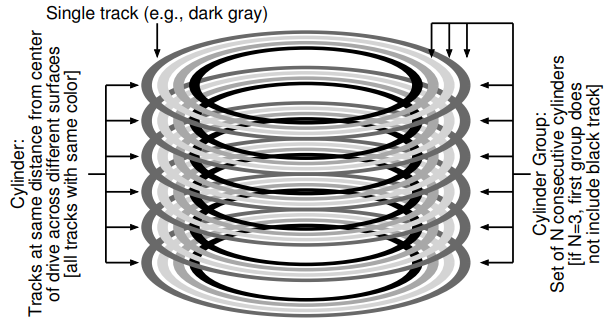
\includegraphics[width=\linewidth]{imgs/ffs_cylinder}
\begin{itemize}
\item FFS keeps same interface/APIs: \texttt{open()},\texttt{read()}, \texttt{write()}, \texttt{close()}, etc
\item disk divided into cylinder groups: A single \mb{cylinder} is a set of tracks on different surfaces of a hard drive with same distance from the center of the drive FFS aggregates $N$ consecutive cylinders into a group
\item modern drives offer limited info for filesys to truly know if a cylinder is in use; disks export logical addr space of blks; hide details of geometry
\item modern sys (ext2-4) organize drive into blk groups: each a consecutive portion of the disk’s addr space; below every 8 blks into one group
  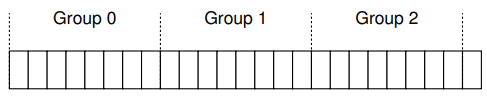
\includegraphics[width=\linewidth]{imgs/ffs_disk_groups}
\item FFS places two files within same group $\to$ ensure that accessing one after the other will not result in long seeks across the disk
\item FFS needs to place files/dir into a group and track all needed info
\item FFS includes all structs a filesys need to have \emph{within} single group
  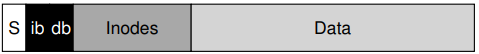
\includegraphics[width=\linewidth]{imgs/ffs_sgroup}
\item FFS keeps a copy of \textbf{S}uperblock to:
  \begin{enumerate*}[label={\arabic*.},font={\color{red!50!black}\bfseries}]
  \item mount the filesys
  \item work as a backup replica if other copies corrupt
  \end{enumerate*}
\item within each group, FFS tracks if inodes/data blks allocated using inode bitmap(ib) and data bitmap(db); inode and data blks same as vsfs
\end{itemize}
\section*{Files and Directories allocation policies}
\begin{itemize}
\item mantra: keep related stuff together; keep unrelated stuff far apart
\item for dirs: find the cylinder group with a low number of allocated directories (to balance directories across groups) and a high number of free inodes (to subsequently be able to allocate a bunch of files), and put the directory data and inode in that group
\item for files:
  \begin{enumerate*}[label={\arabic*.},font={\color{red!50!black}\bfseries}]
  \item make sure to allocate data blocks of a file in the same group as its inode $\to$ prevent long seeks between inode and data
  \item place all files that're in same directory in the cylinder group of the directory they are in:  user creates 4 files, \texttt{/a/b}, \texttt{/a/c}, \texttt{/a/d}, \texttt{b/f}, FFS would try to place 1st three in same group; the 4th far away in some other group
  \end{enumerate*}
\end{itemize}
\begin{minipage}{.5\linewidth}
  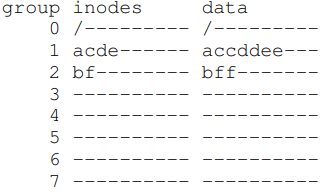
\includegraphics[width=\linewidth]{imgs/ffs_policy1}
\end{minipage}
\begin{minipage}{.5\linewidth}
  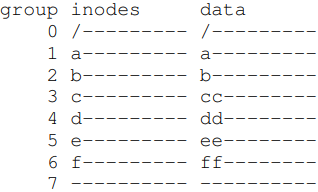
\includegraphics[width=\linewidth]{imgs/ffs_policy2}
\end{minipage}
\begin{itemize}
\item assume 10 inodes and 10 data blocks in each group in above example
\item 3 dirs: \texttt{/}, \texttt{/a}, \texttt{/b} and 4 files: \texttt{/a/c},\texttt{/a/d},\texttt{/a/e},\texttt{/b/f}, each 2 blocks in size
\item \texttt{acde} $\to$ \texttt{/a}, \texttt{a/c}, \texttt{a/d}, \texttt{a/e} (all in Group 1); \texttt{bf} $\to$ \texttt{/b}, \texttt{b/f} in Group 2
\item FFS policy (left):
  \begin{enumerate*}[label={\arabic*.},font={\color{red!50!black}\bfseries}]
  \item places the data blocks of each file near each file’s inode
  \item place files in the same directory near one another
  \end{enumerate*}
\item policy (right) spreads inodes across groups, trying to ensure that no group’s inode table fills up quickly:
  \begin{enumerate*}[label={\arabic*.},font={\color{red!50!black}\bfseries}]
  \item keep file/directory data near its respective inode
  \item files within a dir arbitrarily spread around disk $\to$ name-based locality not preserved: access to \texttt{a/c}, \texttt{a/d}, \texttt{a/e} spans \emph{three} groups instead of \emph{one} per FFS approach
  \end{enumerate*}
\item FFS is based on common sense instead of extensive studies of filesys
\end{itemize}
\section*{Measuring File Locality}
\begin{minipage}{.5\linewidth}
  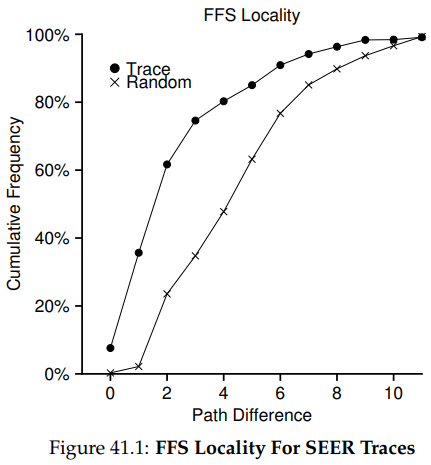
\includegraphics[width=\linewidth]{imgs/ffs_locality}
\end{minipage}
\begin{minipage}{.5\linewidth}
\begin{itemize}
\item if open \texttt{f} first, reopen it next time before any other files $\to$ distance between the 2 opens in dir tree is \textbf{0} (same file)
\item if open \texttt{dir/f}, then open \texttt{dir/g}, distance between the 2 file accesses is \textbf{1} (same dir, different file)
\item metric:
  \begin{enumerate*}[label={\arabic*.},font={\color{red!50!black}\bfseries}]
  \item the longest path to the closest common ancestor of the two files
  \item the closer they are in the tree, the lower the metric
  \end{enumerate*}
\item $\approx$7\% of file accesses were to the file opened previously
\item $\approx$40\% of file accesses were to same file or file in same dir
\end{itemize}
\end{minipage}
\begin{itemize}
\item $\approx$25\% file accesses had a distance of \textbf{2}: when the user has structured a set of related directories in a multi-level fashion and consistently jumps between them: In \texttt{proj/}, jumps between \texttt{proj/src/} and \texttt{proj/obj}
\item FFS does \emph{not} capture this type of locality in its policies $\to$ more seeking
\item random shows less locality but still some $\because$ all files share same root
\end{itemize}
\section*{The large file exception in FFS (the first to intro long file names)}
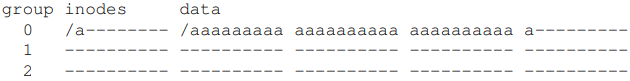
\includegraphics[width=\linewidth]{imgs/ffs_large_file}
\begin{itemize}
\item large file may fill entire block group it's first placed within and others
\item undesired $\because$ other subsequent related data can't be placed in this group
\end{itemize}
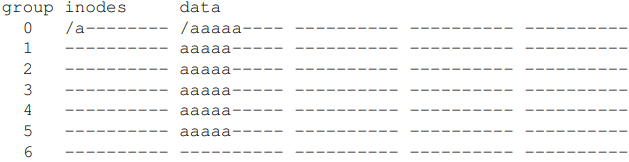
\includegraphics[width=\linewidth]{imgs/ffs_large_file2}
\begin{itemize}
\item with large-file exception, FFS
  \begin{enumerate*}[label={\arabic*.},font={\color{red!50!black}\bfseries}]
  \item alloc some blocks into 1st block group (12 blocks or or \# of direct pointers available within an inode)
  \item places next ``large'' chunk of the file (pointed to by the 1st indirect block) in another block group (maybe chosen for its low utilization)
  \item the next chunk of the file placed in yet another different block group and so on
  \end{enumerate*}
\item related data spread across disk again $\to$ need to use \mb{amortization}: reduce an overhead by doing more work per overhead paid
\item  if the $S_{\text{chunk}}$ large enough, filesys will spend most of its time transferring data from disk and just a relatively little time seeking blk chunks \end{itemize}
\begin{minipage}{.45\linewidth}
  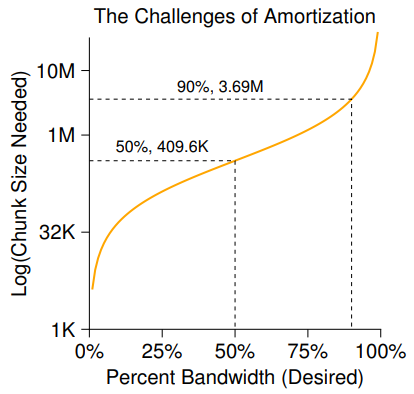
\includegraphics[width=\linewidth]{imgs/ffs_amortization}
\end{minipage}
\begin{minipage}{.55\linewidth}
  \flushleft
  \begin{itemize}
  \item assume avg positioning time (seek + rot.) = 10ms; transfer rate = 40MB/s
  \item goal: 50\% time seeking btwn chunks, 50\% time transferring data $\to$
  \item need spend 10ms transferring data for every 10ms positioning
  \item $\frac{40\;\cancel{MB}}{sec}\cdot\frac{1024\;KB}{1\;\cancel{MB}}\cdot\frac{1\;\cancel{sec}}{1000\;\cancel{ms}}\cdot 10ms = 409.6KB$ transfer amt each time seek
  \item if 90\% peak bandwidth $\to$ trans 3.6MB; if 99\% peak $\to$ trans 39.6MB;
  \item the closer to peak, the bigger chunks
  \end{itemize}
\end{minipage}
\begin{itemize}
\item FFS places:
  \begin{enumerate*}[label={\arabic*.},font={\color{red!50!black}\bfseries}]
  \item 1st twelve blks in same group as the inode
  \item each subsequent indirect blks and all blocks it pointed to in different group
  \end{enumerate*}
\item 4KB block size, 32-bit disk addr $\to$ every 1024 blk (4MB) placed in separate groups, lone exception: first 48KB pointed to by direct ptr
\end{itemize}
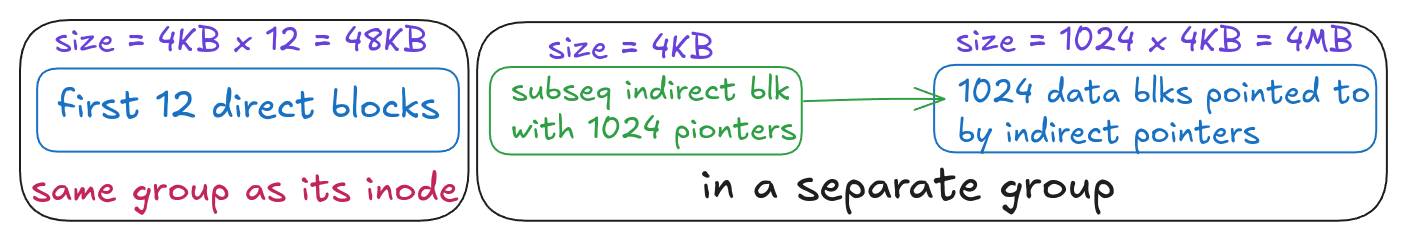
\includegraphics[width=\linewidth]{imgs/ffs_large_file_real}
\begin{itemize}
\item transfer rate $\uparrow$ rapidly $\because$ disk-makers put more bits into same interface
\item mechanical aspects of drives related to seeks (disk arm speed and rotation rate) $\uparrow$ slowly:
  \begin{enumerate*}[label={\arabic*.},font={\color{red!50!black}\bfseries}]
  \item over time mechanical costs become relatively more expensive
  \item transfer more data between seeks to amortize costs
  \end{enumerate*}
\item \mo{interal fragmentation}: FFS uses 512-byte \mb{sub-blocks} to alloc to files
\item 1KB small files needs 2 blks, not 4; as file grows, fielsys alloc more until reaching 4KB of data; at that point, FFS will find a 4KB block, copy the sub-blocks into it, and free the sub-blocks for future use (inefficient)
\item FFS generally avoids this pessimal method and buffer writes until 4KB
\item Modern file systems such as ext2/ext3/ext4 do not allow sub-blocks
\end{itemize}
\begin{minipage}{.45\linewidth}
  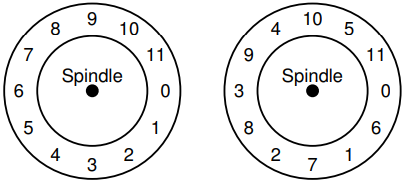
\includegraphics[width=\linewidth]{imgs/ffs_disk_layout}
\end{minipage}
\begin{minipage}{.55\linewidth}
  \flushleft
  \begin{itemize}
  \item left: read 0, wait for completion; then read 1 $\to$ too late as 1 has passed and need to wait for full rotation
  \item right: FFS uses \mb{parameterization} to figure out specific performance params and \# of blks to skip
  \end{itemize}
\end{minipage}
\begin{tcolorbox}[left=0mm, top=1mm, right=0mm, rightlower=0mm, bottom=1mm,
  title= Make System Usable,
  halign title=center]
  FFS was the 1st to intro long file names (more expressive), symbolic links; it also intro atomic \texttt{rename()} to rename files.
\end{tcolorbox}
